\documentclass[11pt]{article}
\usepackage{coling2014}
\usepackage{times}
\usepackage{url}
\usepackage{latexsym}
\usepackage{graphicx}

%\setlength\titlebox{5cm}

% You can expand the titlebox if you need extra space
% to show all the authors. Please do not make the titlebox
% smaller than 5cm (the original size); we will check this
% in the camera-ready version and ask you to change it back.


\title{CLAM: Quickly deploy NLP command-line tools on the web}

\author{Maarten van Gompel \\ 
  Centre for Language Studies (CLS) \\
  Radboud University Nijmegen \\
  {\tt proycon@anaproy.nl } \And 
  Martin Reynaert \\
  CLS, Radboud University Nijmegen \\
  TiCC, Tilburg University  \\
  {\tt reynaert@uvt.nl } 
  }

\date{}

\begin{document}
\maketitle

\begin{abstract}
In this paper we present the software CLAM; the Computational Linguistics
Application Mediator. CLAM is a tool that allows you to quickly and
transparently transform command-line NLP tools into fully-fledged
\emph{RESTful}\/ webservices with which automated clients can communicate, as
well as a generic webapplication interface for human end-users.
\end{abstract}


\section{Introduction}

In the field of Natural Language Processing, the majority of tools come in the
form of command-line tools aimed at UNIX-derived systems. We consider this good
practice in line with the UNIX philosophy \cite{unixphilo} which states,
amongst others, that programs should 1) do one thing and do it well, and 2) expect the output of one
program to be the input of another. This can be rephrased as the \emph{Rule of
Modularity}, write programs consisting of simple parts, connected by
well-defined interfaces \cite{RAYMOND2004}.

Programs operating at the command-line
offer such modularity, making them ideally suitable for integration in a
wide variety of workflows. However, the command-line may not be the most suitable interface for non-specialised
human end-users. Neither does it by itself facilitate usage over network unless
explicit server functionality has been programmed into the application.
Humand end-users often want a Graphical User Interface (GUI), a special instance of which
being a Web User Interface. Yet for automated clients operating over a network, such an interface is a
cumbersome barrier, and they instead prefer a properly formalised webservice
interface. CLAM offers a solution to this problem, when all there is is a
simple NLP command-line tool.

CLAM finds application in areas where people want to make their software
available to a larger public, but a command-line interface is not sufficient.
Setting up your tool may be complicated, especially if there are many
dependencies or the target audience does not use linux machines. CLAM is
ideally suited for quick demo purposes, or for integration into larger workflow
systems. It removes the burden from the software developer (you) to have to
implement a service mode and build a GUI or web-interface, thus saving precious
time.

\section{System architecture}

The Computational Linguistics Application Mediator (CLAM) is a tool that wraps
around your command-line interface and allows you to very quickly and
transparently turn your program into \textbf{1)} a \emph{RESTful}\cite{REST} webservice with which
automated clients can communicate, as well as \textbf{2)} a generic web user interface
for human end-users. Just like an actual clam is a
shell around the animal that inhabits it, which most never see
directly, CLAM wraps around your sofware, providing extra functionality and
hardening it through its built-in security mechanism. You do not need to modify
your original software in any way, it is always taken as a given, you merely
need to describe it. 

An NLP command-line tool can usually be described in terms of \emph{input
files}, \emph{output files} and parameters influencing its run. Parameters may
either be \emph{global parameters}, pertaining to the system as a whole, or
\emph{local parameters} which act as metadata for specific input files. File
formats are never dictated by CLAM itself, but are up to the service provider
to define.

CLAM discerns three \emph{states}, which also reflects the stages in which
the end-user or automated client interacts with he system

\begin{enumerate}
  \item The system is ready to accept files for input and input parameters
  \item The system is running
  \item The system is done and the output files are offered for
    presentation/download.
\end{enumerate}

Any tool that can be described in these terms can be used with CLAM. The system
has been designed specifically to work with software that may take quite some
time to process or runs large batches. Stage two therefore is not confined to
lasting mere seconds as is custom in web-based applications, but may last as
long as hours, days, or any duration that the end-user is willing to wait.
Also, end-users need not maintain a connection to the server. Human end-users
may close their browser and return at will, and automated clients simply poll the
system's status with a certain interval.

You are not limited to just a single run of your system; you may set it up to
allow upload and processing of multiple files and run them in batch fashion.
This approach is common in processing text files for purposes such as
tokenisation or any form of tagging.

In order for CLAM to turn a command-line tool into a webservice, developers are
expected to provide two things in addition to the actual tool: 

\begin{enumerate}
  \item \textbf{Service configuration} - This specifies everything there is to
    know about your application, it defines what the input will be, what
    the output will be, and what parameters the system may take. Input and output
    are always in the form of files. The web user interface, however, also
    optionally offers a text field for users to create files on the fly.
    
  \item \textbf{System wrapper script} - This is a small script that CLAM will
    invoke to start your system. It acts as the glue between CLAM and your
    actual application and may do some necessary interpretation and
    transformation of parameters to suit the command-line interface of your
    application.
\end{enumerate}

A generic client for communicating with the webservice is already provided,
more specific clients can be written using the CLAM API (Python) to greatly
facilitate development.

The architecture is visualised in the scheme in Figure~\ref{fig:arch}.

\begin{figure}[h]
\begin{center}
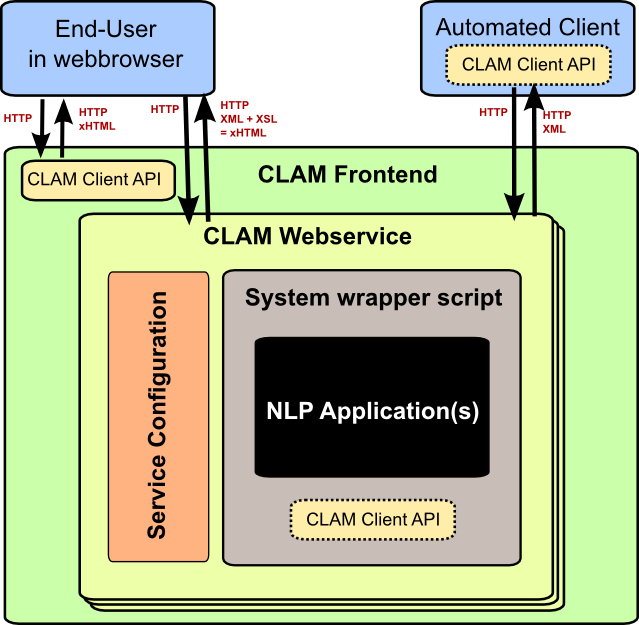
\includegraphics[width=100.0mm]{architecture.png}
\end{center}
\caption{Schematic overview of the CLAM architecture}
\label{fig:arch} 
\end{figure}

CLAM is a multi-user system, although out-of-the-box it simply uses an
``anonymous'' user and requires no authentication. Each user can create an
arbitrary number of \emph{projects}. One project corresponds to one run of the
system, which may be one large batch depending on how you configure your
service. Users can always return to earlier projects and inspect input files
and output files, until they explicitly delete the project.

The strong metadata support in CLAM has to be emphasised as one of it's notable
features. Metadata can be associated with any input files, and the profiles in
the service configuration file determines how such metadata is carried over to
output files. Additionally, as part of the metadata, provenance data is
generated for all output files. This occurs in a simple and straightforward XML
format.

\section{Extensions}

CLAM can be extended by developers in several ways. One is to write
\emph{viewers}, which take care of the visualisation of output files for a
specific file format, and are used by the web user interface. Viewers may be
implemented as internal Python modules, or you can link to any external URL
which takes care of the visualisation. Another extension is
\emph{converters}, these allow users to upload an input file in one file-type and have it
automatically converted to another. Converters for PDF and Word to plain text are already
provided through the tools \texttt{pdf2txt} and \texttt{antiword}.

\section{Technical Details}

CLAM is written in Python (2.6 or 2.7), \cite{PYTHON}. It comes with a built-in HTTP server for
development purposes, allowing you to quickly test and adjust your service.
Final deployment can be made on common webservers such as Apache, Nginx or lighthttpd
through the WSGI mechanism. The service configuration file itself is by
definition a Python file calling specific configuration directives in the CLAM
API. The system wrapper script may be written in any language, but Python users
benefit as they can use the CLAM API which makes the job easier. Projects and
input files are stored in a simple directory structure on disk, allowing your
tool easy access. No database server is required.

The webservice offers a \emph{RESTful} interface \cite{REST}, meaning that the HTTP
verbs \texttt{GET}, \texttt{POST}, \texttt{PUT} and \texttt{DELETE} are used on
URLs that represent resources such as projects, input files, output files. The
web application is implemented as a client-side layer on the webservice. It is
presented through XSL transformation \cite{XSLT} of the webservice XML output.

User authentication is implemented in the form of HTTP Digest Authentication,
which ensures that the password is sent in encrypted form over the network even
with servers where HTTPS is not used. HTTPS support is not present in CLAM
itself but can be configured in the encompassing webserver. The underlying user
database can be specified either directly in the service configuration file or
in a table in a Mysql database, but it is fairly easy to replace this and
communicate with another external database of your choice instead. There is
also support for being relayed credentials from another authentication source
such as Shibboleth, allowing for integrating with single-sign-on scenarios.
Implementation of OAuth2 will follow in a later version.

CLAM is open-source software licensed under the GNU Public License v3.

\section{Related Work}

As far as we know, the only tool comparable to CLAM is Weblicht
\cite{WEBLICHT}. Both tools are specifically designed for an NLP context. CLAM,
however, is of a more generic and flexible nature and may also find easier
adoption in other fields.

When it comes to data formats, Weblicht commits to a specific file format for
corpus data. CLAM leaves file formats completely up to the service providers,
although it does come, as a bonus, with a viewer for users of FoLiA \cite{FOLIA}.

Weblicht is Java-based whereas CLAM is Python-based, which tends to be less
verbose and more easily accessible. System wrapper scripts need not even be
written in Python if the developer prefers another language, and service
configuration files simply consist of directives that requires virtually
no Python knowledge.

All in all CLAM offers a more lightweight solution than Weblicht, allowing
webservices to be set-up more easily and quicker. Nevertheless, CLAM offers
more power and flexibility in doing what it does: wrapping around command-line
tools, its webservice specification is more elaborate than that of Weblicht. On
the other hand, CLAM deliberately does not go as far as Weblicht and does not
offer a complete chaining environment, which is what Weblicht is. In this we
follow the aforementioned UNIX philosophy of doing one thing well and one thing
only. Service chaining certainly remains possible and CLAM provides all the
information to facilitate it, but it is left to other tools designed for the
task. CLAM has been successfully used with Taverna \cite{TAVERNA} in the scope
of the CLARIN-NL project ``TST Tools for Dutch as Webservices in a Workflow''
\cite{KEMPSSNIJDERS2012}. 

\section*{Acknowledgements}

CLAM support and development is generously funded by CLARIN-NL \cite{CLARIN}, and is being
used by various projects in the Dutch \& Flemish NLP community, whose feedback
and support have contributed to its success. 

% include your own bib file like this:
\bibliographystyle{acl}
\bibliography{clam}


\end{document}
